%%
%% Copyright 2007, 2008, 2009 Elsevier Ltd
%%
%% This file is part of the 'Elsarticle Bundle'.
%% ---------------------------------------------
%%
%% It may be distributed under the conditions of the LaTeX Project Public
%% License, either version 1.2 of this license or (at your option) any
%% later version.  The latest version of this license is in
%%    http://www.latex-project.org/lppl.txt
%% and version 1.2 or later is part of all distributions of LaTeX
%% version 1999/12/01 or later.
%%
%% The list of all files belonging to the 'Elsarticle Bundle' is
%% given in the file `manifest.txt'.
%%
%% Template article for Elsevier's document class `elsarticle'
%% with harvard style bibliographic references
%% SP 2008/03/01

% \documentclass[preprint,12pt,authoryear]{elsarticle}
\documentclass[final,twocolumn,3p,times,authoryear]{elsarticle}

%% Use the option review to obtain double line spacing
%% \documentclass[authoryear,preprint,review,12pt]{elsarticle}

%% Use the options 1p,twocolumn; 3p; 3p,twocolumn; 5p; or 5p,twocolumn
%% for a journal layout:
%% \documentclass[final,1p,times,authoryear]{elsarticle}
%% \documentclass[final,1p,times,twocolumn,authoryear]{elsarticle}
%% \documentclass[final,3p,times,authoryear]{elsarticle}
%% \documentclass[final,3p,times,twocolumn,authoryear]{elsarticle}
%% \documentclass[final,5p,times,authoryear]{elsarticle}
%% \documentclass[final,5p,times,twocolumn,authoryear]{elsarticle}


\usepackage[utf8]{inputenc}



%% For including figures, graphicx.sty has been loaded in
%% elsarticle.cls. If you prefer to use the old commands
%% please give \usepackage{epsfig}

%% The amssymb package provides various useful mathematical symbols
\usepackage{amssymb}
\usepackage{color}
\usepackage{url}
\usepackage{hyperref}
\usepackage{graphicx,array}
\usepackage{amsmath}
\usepackage{siunitx}
\usepackage{bm}
\usepackage{aasmacros}

%% The lineno packages adds line numbers. Start line numbering with
%% \begin{linenumbers}, end it with \end{linenumbers}. Or switch it on
%% for the whole article with \linenumbers.
%% \usepackage{lineno}

\newcommand{\nati}[1]{{\color[rgb]{.1,.6,.1}{#1}}}

\newcommand{\todo}[1]{{\color[rgb]{.6,.1,.6}{#1}}}

\newcommand{\assign}[1]{{\color[rgb]{.8,.5,.8}{Assigned: #1 }}}


\renewcommand{\b}[1]{{\bm{#1}}}   % bold symbol

% MATH SYMBOLS
\newcommand{\1}{\b{1}}              % all-ones vector
\newcommand{\0}{\b{0}}              % all-zero vector
\newcommand{\g}[1]{\b{#1}}
\renewcommand{\L}{\b{L}} % the laplacian matrix
\newcommand{\W}{\b{W}}
\newcommand{\I}{\b{I}}
\newcommand{\D}{\b{D}}
\newcommand{\U}{\b{U}}
\newcommand{\bLambda}{\b{\Lambda}}
\newcommand{\blambda}{\b{\lambda}}
\newcommand{\pkg}[1]{\texttt{#1}}


\journal{Astronomy and Computing}

\begin{document}

\begin{frontmatter}

%% Title, authors and addresses

%% use the tnoteref command within \title for footnotes;
%% use the tnotetext command for theassociated footnote;
%% use the fnref command within \author or \address for footnotes;
%% use the fntext command for theassociated footnote;
%% use the corref command within \author for corresponding author footnotes;
%% use the cortext command for theassociated footnote;
%% use the ead command for the email address,
%% and the form \ead[url] for the home page:
%% \title{Title\tnoteref{label1}}
%% \tnotetext[label1]{}
%% \author{Name\corref{cor1}\fnref{label2}}
%% \ead{email address}
%% \ead[url]{home page}
%% \fntext[label2]{}
%% \cortext[cor1]{}
%% \address{Address\fnref{label3}}
%% \fntext[label3]{}

\title{HealpixNet: Efficient spherical Convolutional Neural Networks with Healpix sampling for cosmological applications}

%% use optional labels to link authors explicitly to addresses:
%% \author[label1,label2]{}
%% \address[label1]{}
%% \address[label2]{}

\author{}

\address{}

\begin{abstract}
%% Text of abstract

Convolutional Neural Networks (CNNs) are becoming an important analysis tool in cosmology and astrophysics.
In many applications, the data comes in a form of spherical maps.
A popular format for these maps is Healpix, which uses equal-area, isolatitude sampling.
We present a CNNs for analysis of full- and partial sky Healpix maps, which we call HealpixCNN (???).
This approach is based on representing a sphere as a graph of connected nodes.
We describe a convolution operation defined on that graph.
HealpixCNN (???) uses Tensorflow as the underlying engine and can utilise most of it functionalities.
Architectures can be designed in a similar way as standard CNNs used for image analysis.
We find that the graph-based convolution is very efficient (MORE HERE)..
The filters learned by the HealpixCNN are restricted to being radial.
We demonstrate the method on a simple classification problem of mass maps from two cosmological models.
We compare the performance to a simple benchmark classifier, which uses histograms of map pixel values.
HealpixCNN achieves much better testing accuracy than the benchmark approach.
We make the code and examples available to the public.

	\todo{(Michaël) I would not invent a new term, SCNN, but rather say that convolutional neural networks on graphs (or GCNs) can be efficiently applied to (spherical?) cosmological applications.
	Arguments: the method is not new and hence don't deserve a new name. Emphasize that it is generic to the data structure, and that the sphere is simply a particular graph.
	Ideas: Graph Convolutional Networks for efficient spherical ???, Efficient spherical ??? with GCNs and Healpix sampling
    We make the code publicly available.
    \\
    \todo{(Tomek) How about HealpixCNN? Or HealpixNet? Or HealNet?}

}

\end{abstract}

\begin{keyword}
%% keywords here, in the form: keyword \sep keyword

%% PACS codes here, in the form: \PACS code \sep code

%% MSC codes here, in the form: \MSC code \sep code
%% or \MSC[2008] code \sep code (2000 is the default)

\end{keyword}

\end{frontmatter}

%% \linenumbers

\section{TODO list}
\begin{itemize}
    \item Michael, do you agree with the title HealpixNet
    \item
\end{itemize}

%% main text
\section{Introduction}
\label{sec:intro}

%\subsection{Motivation}
\assign{Tomek}

Cosmological and astrophysical data often comes in a form of spherical sky maps.
Observables that cover large parts of the sky, such as the Cosmic Microwave Background (CMB) \citep{planck2015cosmologicalparameters,komatsu2011sevenyear,staggs2018recentdiscoveries}, neutral hydrogen \citep{santos2015cosmologySKA,HI4PI2016fullskyHI}, galaxy clustering \citep{alam2017clusteringgalaxies}, gravitational lensing \citep{troxel2017darkenergy,hildebrandt2017kidscosmological}, and others, have been used to constrain cosmological and astrophysical models. Deep Learning methods have recently started to gain popularity as an analysis tool in cosmology \citep{schmelze2017cosmologicalmodel,luciesmith2018machinelearning,gupta2018nongaussianinformation,gillet2018deeplearning,hassan2018reionizationmodels,aragoncalvo2018classyfyinglarge,ciuca2017cnnstring}.
Convolutional Neural Networks (CNNs) are particularly well suited for analysis of astrophysical data due to their ability to capture complicated, non-linear patterns, which are often present in the data.

So far these algorithms have been demonstrated on the flat images.
Deep learning-based analysis of larger survey area form requires dividing the data into smaller chunks and projecting them on a flat, 2D surface.
While this process can work efficiently as already demonstrated, it may be more convenient do work with deep learning directly on the sphere.
The most commonly used scheme in astrophysics to divide a sphere into pixels is Healpix \citep{gorski2005healpix}, which uses isolatitude sampling and pixels with the same area.

In this work we present an algorithm and software package \pkg{SCNN-temp-name}\footnote{github.com/SwissDataScienceCenter/scnn} which implements efficient deep convolutional neural networks on Healpix maps.
To achieve this, we represent the sphere $S^2$ as a graph of connected pixels, which forms a 2D manifold embedded in 3D space $\mathbb{R}^3$.
This approach is based on CNN formulations on graphs described by \citet{defferrard2016convolutional} and runs using the \pkg{TensorFlow} \citep{abadi2016tensorflow} engine.
The flexibility of the graph approach allows for faster analysis when data spans only a part of the sphere.
It is also possible to use multiple Healpix maps within our framework and use datasets in form of ``shells''.
These shells can span the radial direction, so that a tomographic analysis can be performed, or different frequencies, in case of data from observations in radio frequencies.

Formulations of deep learning on the sphere have been proposed by ~\citet{cohen2017convolutional,cohen2018spherical}.
In that method, a different sphere pixelisation scheme is used: the sphere pixels are mapped to flat space (??) and then generalized Fast Fourier Transform (FFT) is used for convolutions.
Other recently developed sampling methods include \citep{mcewen2011novelsampling}, where exact sampling theorem for equiangular MW sampling was presented.
In our work we focused on the Healpix sampling, as it is the most commonly used in cosmology.
It can be, however, extended to other sampling schemes, by straightforward change in definition of the graph.

Another advantage of our method is the speed of the convolution operation.
It is the most efficient spherical convolution\footnote{\todo{provably? cannot be faster than O(n) without approximations, e.g. sketching}}, requiring only $O(n)$ operations, where $n$ is the number of points.
MORE HERE

The method presented here restricts the shape of the filters learned by the network to be radial.
While this may be a less general design compared to the one used by conventional CNNs on flat images, we found it to still work efficiently for our test cases.
The layered structure of the network can partially compensate for that.
Further generalisations to non-radial filters may be possible [cite?], but we leave it to future work.

We give a practical demonstration of the application of our package to cosmological model discrimination using convergence maps, similar to \citep{schmelze2017cosmologicalmodel}.
In a simplified scenario, we classify convergence maps on parts of a sphere into two cosmological models.
These models were designed to have the same power spectrum in range $\ell < 1000$.
We compare the performance of the spherical CNN to a baseline algorithm, a SVM classifier which takes pixel histograms of these maps as input.
The comparison is made as a function of noise level on convergence maps and area of the sphere used.

The paper is organised as follows.
In Section \ref{sec:related} we describe existing approaches to convolutions on the sphere, graphs, and manifolds.
Section \ref{sec:method} we show the way to construct a graph using Healpix sampling and define the convolution operation.
The comparison between the spherical CNN and the benchmark method using the weak lensing mass map classification is presented in Section \ref{sec:experiments}.
We conclude in Section \ref{sec:conclusion}.
% Cite the following papers:
% \begin{itemize}
%     \item Healpix paper \citep{gorski2005healpix}
%     \item First DES mass maps \citep{chang2017curvedsky}
%     \item Healpix convolutions with asymetric beams \citep{mitra2011fastpixel}
%     \item Mass mapping on the sphere \citep{wallis2017mappingdark}
%     \item Wavelets on the sphere \citep{leistedt2016wavelet} and ball \citep{leistedt2012exactwavelets}
%     \item Planck main result \citep{planck2015cosmologicalparameters,komatsu2011sevenyear}
%     \item HI map \citep{HI4PI2016fullskyHI,}
%     \item more radio maps from Adam+Hamsa \citep{santos2015cosmologySKA}
%     \item more astro science on the sphere, what other survey make maps?
%     \item alternative sampling on the sphere \citep{mcewen2011novelsampling} MW sampling
%     \item cite kids tomographic power spectrum \citep{koehlinger2017kidstomographic}
% \end{itemize}


% a) Cosmology has a lot of spherical data. Our method is simple and easy to use. Moreover, it is based on the widely used healpix sampling.
% b) It is the most efficient spherical convolution\footnote{\todo{provably? cannot be faster than O(n) without approximations, e.g. sketching}}, requiring only $O(n)$ operations, where $n$ is the number of points.

% \subsection{Potential applications}
% 	\assign{Tomek, Nathanaël, Michaël}

% The analysis of spherical cosmological data, such as the cosmic microwave background \cite{...}, as done in \cite{he2018analysis}, is the target application of our method.

% While our method was developed with cosmology in mind, it can easily target any problem where data live on a sphere. Examples include, but are certainly not limited to, (i) efficient compression and decompression of \ang{360} videos (see \cite{su2017learning}), (ii) \todo{data analysis on planets? (climate, forecasting, temperature, wind)}, (iii) \todo{particle physics? (jets on detectors, but they are usually cylindrical)}, (iv) \todo{applications in Cohen's papers?}.

% Finally, not that those neural networks are not restricted to the sphere and can be applied to any problem where we have data on a graph, such as social, biological or infrastructure networks [some citations, e.g. brain Alzeihmer, particle physics, computer graphics].
% the convolution is not restricted to the sphere, the coarsening/pooling is


% \section{Healpix sampling}
% Should we have this subsection to explain the advantages of Healpix?
% \begin{itemize}
% 	\item Define the spherical grid?
% 	\item reference the "cubed sphere"~\cite{ronchi1996cubed}?
% \end{itemize}

% \begin{figure}[!ht]
% \centering
% 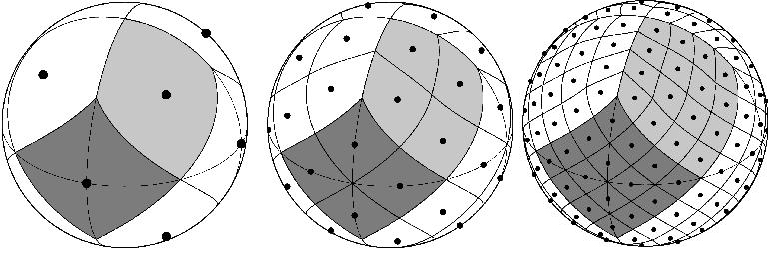
\includegraphics[width=0.45\textwidth]{figures/healpix-3layers.jpg}
% \caption{3 smaller sclales of the healpix sampling.}
% \label{fig:healpix_sampling}
% \end{figure}

\section{Related work}
\label{sec:related}



\subsection{Spherical convolutions}
The major challenge to define Convolution Neural Network (CNN) onto a
spherical domain is to handle a convolution that is suitable for this irregular sampling domain.
Three approaches exist to address this issue.

The first approach, leveraging the continuous spherical convolution, has been
proposed by~\cite{cohen2017convolutional,cohen2018spherical}. The goal of these
contributions it to use a rotational equivariant convolution on the
sphere, i.e. a rotation of the input implies the same rotation of the output.
The resulting convolution is performed by a spherical Fourier transform (i.e. a projection
on the spherical harmonics), a  multiplication in the spectral domain and an
inverse spherical Fourier transform. Hence the main computational cost of a
convolution comes from the two Fourier transforms. Fortunately, the Fourier
transform can be accelerated for special samplings set (theoretically including
HealPix, \cite{...}). The main advantage of this approach is that it provides a
mathematically well defined rotational equivariant network. Nevertheless, even
with these Fourier transform acceleration, the convolutions remain expensive in
comparison to a traditional 2-dimensional convolution, limiting the practical use of this
approach. While a comparison is theoretically possible, the experiments
of~\cite{cohen2018spherical} are done using the geodesic grid sampling set and
do not provide any code for the Healpix one. Hence, a practical comparison is
not possible.

A second direction has been followed in~\cite{boomsma2017spherical}. The idea is
to use the traditional 2-dimensional convolution on an irregular grid defined on the
sphere. In the paper, two grids are used: the geodesic grid and the “cubed
sphere” grid defined by Ronchi et. al~\cite{ronchi1996cubed}. Because this
approach is based on the traditional 2-dimensional convolution, it is very likely to be the
most efficient one. However, it suffers that it can only be used using very
specific grid sampling sets which are NOT including HealPix. Furthermore, the
grid requirement makes it impossible for the convolution to capture the
spherical properties of the domain, i.e. the "cubed sphere” sampling is by
definition adapted to a cube and not to a sphere.
% \nati{Michael: Under some very
% specific hypothesis, this second approach is a particular case of our method,
% i.e. 1) our method with a stupid sampling, 2) assumption that graph convolution
% on a grid == 2d convolution. Do you think we should mention that? I think we
% should not.}

In an attempt to get the best of the two first approaches, we follow a third
direction. We use a graph to adapt to the particular structure of the sphere.
While the convolution remains efficient, it still captures well the spherical
structure and is particularly adapted to the HealPix sampling.

We are not the first one to leverage a graph to define a CNN on a sphere.
\cite{khasanova2017graph} use the same idea to handle omnidirectional images.
Besides the different application covered by the paper, there are two important
differences. First the sampling is different as \cite{khasanova2017graph} uses a
grid. Second, it uses a different graph CNN based on a different parametrisation
of the convolution kernel.


\subsection{Convolutions on graphs}
\assign{Michaël}

\todo{other approaches? GNNs, Kipf first order approx, message passing}

Previous work: [Bruna] which needed the full eigendecomposition of the Laplacian, costing $O(n^3)$ operations.

In this work, we are using the graph CNN formulation introduced in~\cite{defferrard2016convolutional}.

Spatial definitions of graph convolutions, e.g. [Niepert] needs to define an orientation in order to match the edges with the filters. Most often the orientation is not given by the application, and one has to define it (for example by ordering by degree or any other measure, or by using a graph coloring). There is no good default good orientation on general graphs and the choice of an orientation is highly application dependent.

\todo{Cool to have a global illustration of the network (CNN like)}

\subsection{Convolutions on manifolds}
\todo{TK and NP: maybe we just describe convolutions on sphere and graph}

Related to this, convolutional neural networks have been defined on manifolds and have achieved impressive results on shapes [Bronstein]. They however too depend on an orientation, which spheres do not possess.

\subsection{Convolutions on point clouds?}
\todo{TK and NP: maybe we just describe convolutions on sphere and graph}

PointNet and co. Related but we are loosing the structure. Also coarsening.

\section{Method}
\label{sec:method}
% \begin{itemize}
% 	\item We build a graph using the healpix sampling
% 	\item Define Fourier transform and show that the harmonics are visually close to the spherical harmonics
% 	\item Define spherical convolution using the graph Fourier transform and show heat diffusion example
% 	\item Show the limits of the approach and explain why we cannot have a perfect spherical convolution with this technique
% \end{itemize}

The gist of our method is to define the convolution on a sphere using a graph.
The graph is here seen as a discrete approximation of the sphere $S^2$, a
2-dimensional manifold embedded in $\mathbb{R}^3$.

As presented by~\cite{cohen2018spherical}, the most mathematical approach to
extend the convolution on a sphere is to use a spherical Fourier transform. The
convolution is then simply defined as the product in the spectral domain. This
approach requires one Fourier and one inverse Fourier transform per convolution
which remain, even with accelerated algorithms, expensive. For 2-dimensional
images, an efficient convolution can be achieved when the convolution kernel is
localized (for example a 5x5 pixel patch) by doing the computation directly in
the signal domain. Unfortunately, this approach cannot be directly extended to
the spherical case. Hence, the main idea of this contribution is to leverage
graph signal processing~\cite{shuman2013emerging} to define a spherical
convolution that can be computed (and back-propagated) directly in the signal domain.

\subsection{Graph creation}
In the classical 2-dimenstional convolution, each pixel is connected with the
same weight to its 4 closest neighbors. We use a weighted undirected graph to
generalize this idea to the ubiquitous HealPix
sampling~\citep{gorski2005healpix}.  Each pixel is represented by a node
(vertex) connected to his $8$ or $7$ closest neighbors.\footnote{For some
pixels, the $8^{th}$ nearest neighbor is not well defined.} Given the set of
nearest neighbors, we define the weight matrix $W$ using the following scheme
\begin{equation}
W[i,j]=\begin{cases}
e^{-\frac{\|x_i-x_j\|_2^2}{\sigma^2}} & \text{if pixels $i$ and $j$ are connected, and}\\
0 & \text{otherwise.}\\
\end{cases}
\end{equation}
Here $x_i$ is a 3-dimensional vector encoding the coordinate of the pixels $i$
on the sphere and $\sigma$ is the mean of $\|x_i-x_j\|_2$ over all connected
pixels $i$ and $j$. This weighting scheme is important as the distances between
pixels varies due to the small sampling irregularities. Some of the
irregularities have been highlighted in the graph displayed in
Figure~\ref{fig:healpix_graph_4}.

These small irregularities are important and affect slightly the degree of a
node (or a pixel), defined as $d_i =\sum_j W[i,j]$.

\begin{figure}[!ht]
\centering
% 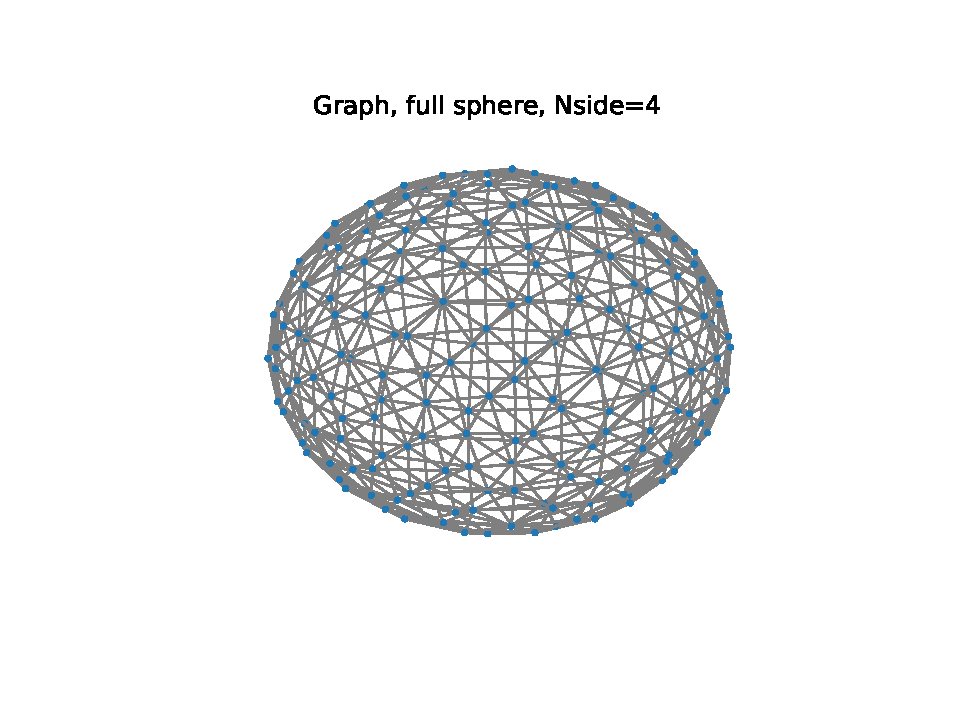
\includegraphics[width=0.45\textwidth]{figures/healpix_graph_4.pdf}
\vspace{-0.5cm}
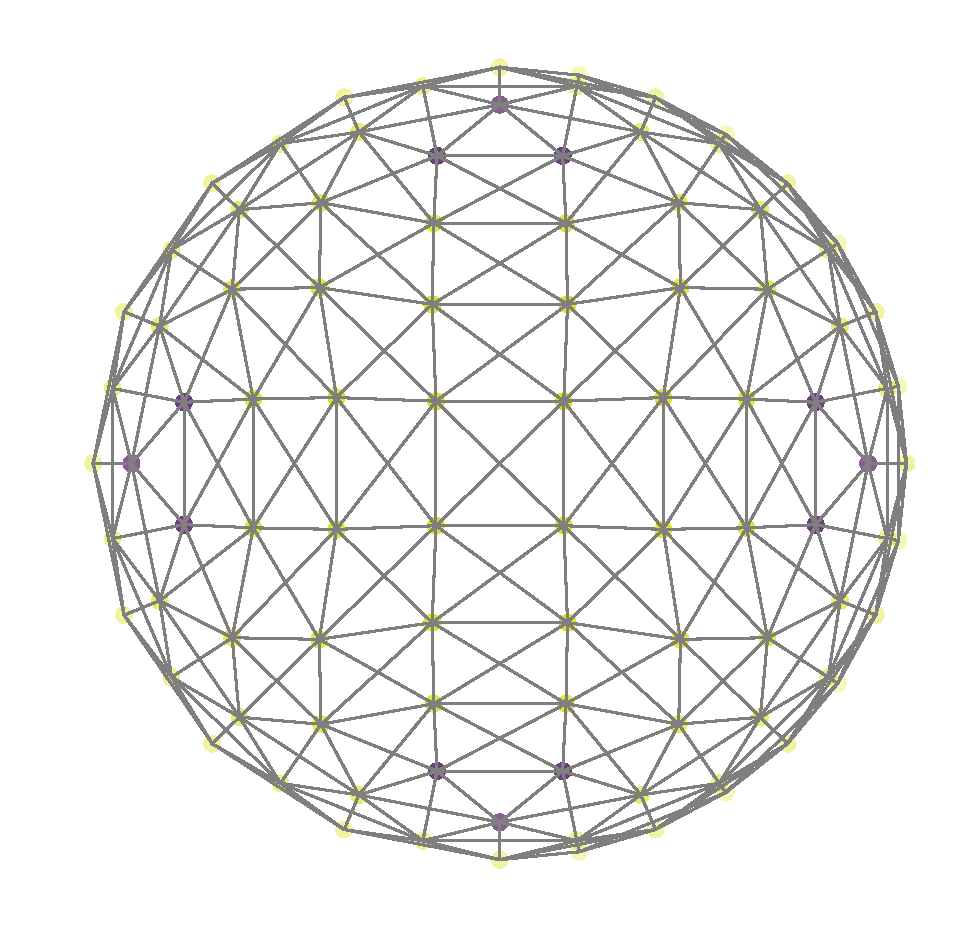
\includegraphics[width=0.45\textwidth]{figures/half_graph_4.pdf}
\vspace{-0.5cm}
\caption{
Top view of a Healpix graph for half the sphere using an nside parameter of $4$.
Nodes with 7 neighbors are highlighted.
}
\label{fig:healpix_graph_4}
\end{figure}

\subsection{Graph Fourier basis and spherical harmonics}
\todo{Add a few extra references}

Because of the irregular sampling, there is no obvious way to define the convolution
directly from the pixel values. Hence we will first make a detour and define a Fourier transform on the
graph.

Following~\cite{shuman2013emerging}, the graph normalized graph Laplacian
defined as $\L = \I - \D^{-1/2} \W \D^{-1/2}$ is a second order differential operator
that can be used to define the graph Fourier basis. Here $D$ is the diagonal
matrix where $\D_{ii}=\b{d}_i$. By construction the Laplacian is symetric positive
semi-definite and hence can be decomposed as $\L=\U \bLambda \U^*$, where $U$ is an
orthonormal matrix of eigenvectors and $\bLambda$, the diagonal matrix of
eigenvalues. The graph Fourier basis is defined as the Laplacian eigenvectors.
The graph Fourier transform of $f$ is simply its projection on $U$ given by
$\hat{\b{f}}=\U^*\b{f}$. Similarly the inverse graph Fourier transform reads $\b{f}=\U\hat{\b{f}}$.
Note that instead of frequencies, the Fourier modes are crescently ordered with
respect of the Laplacian eigenvalues $\bLambda$. In a sense, the Laplacian
eigenvalues correspond to the squared frequencies.

\begin{figure*}[!ht]
\centering
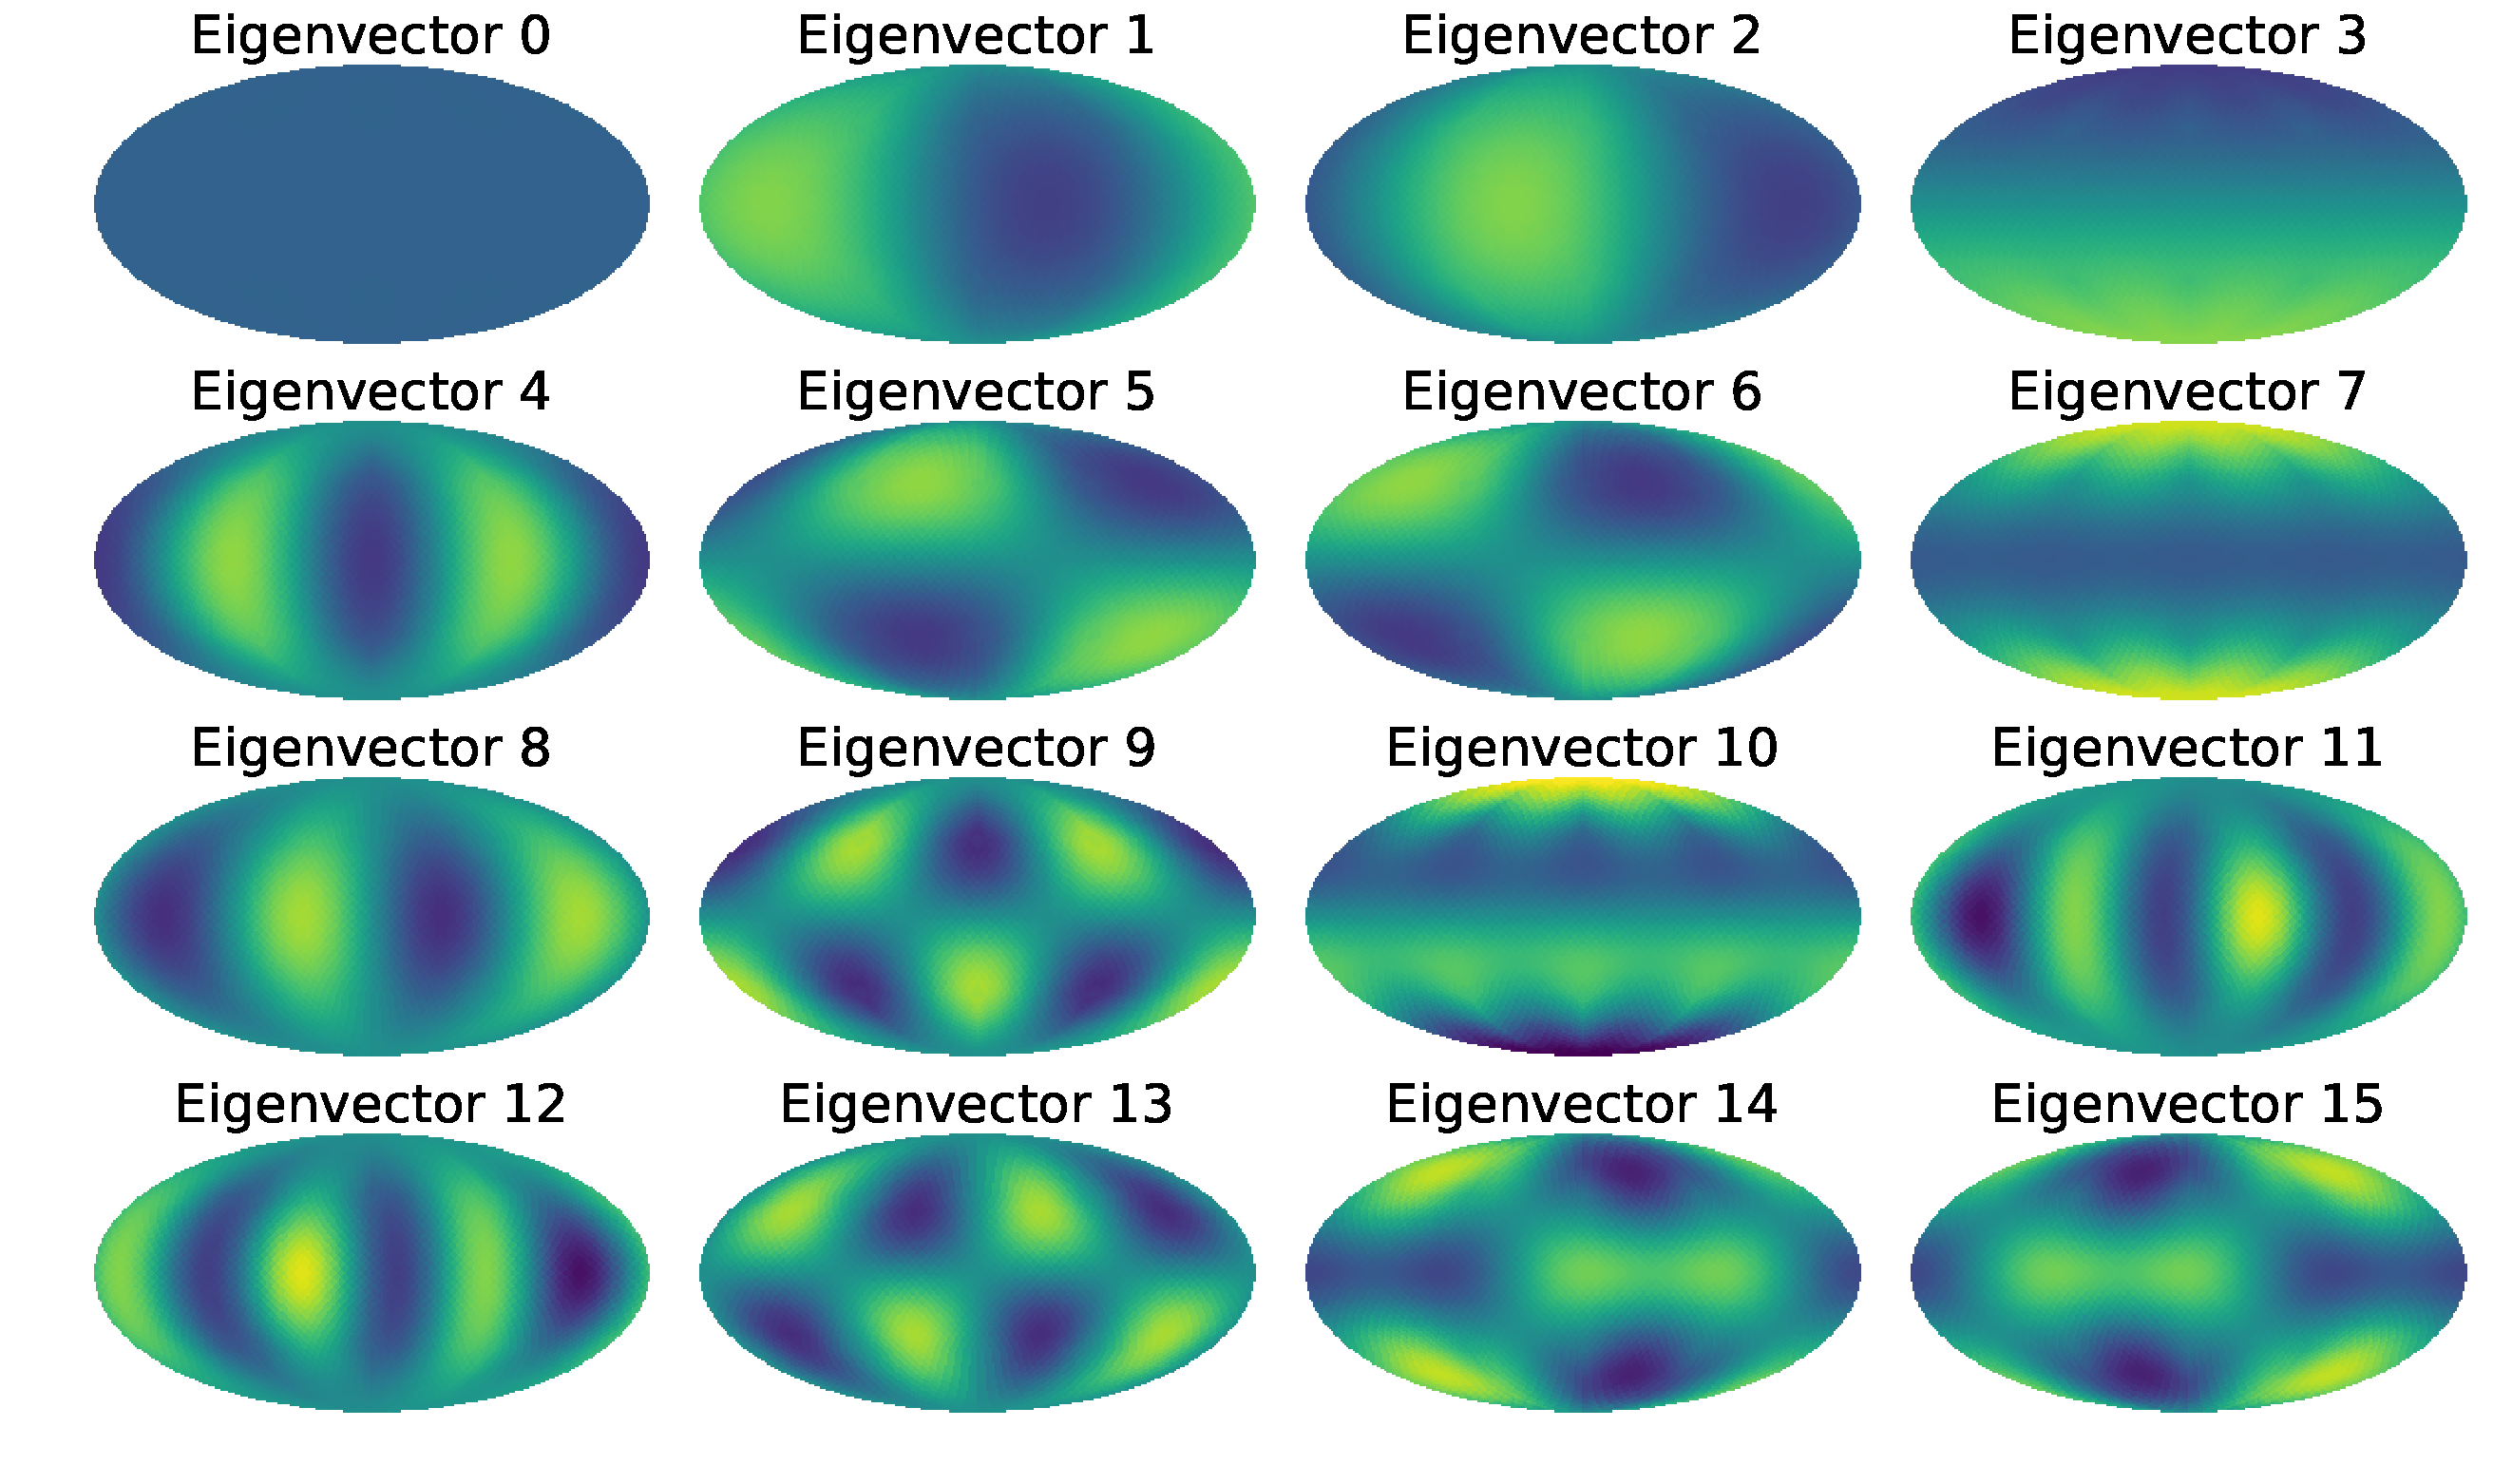
\includegraphics[width=0.95\textwidth]{figures/eigenvectors.pdf}
\caption{12 first graph Fourier eigenvectors.}
\label{fig:graph_harmonics}
\end{figure*}

As shown in Figure~\ref{fig:graph_harmonics}, it turns out that using the graph
construction described above, the graph Fourier harmonics resemble the
classical spherical harmonics giving us an indication that the graph is able to
capture the spherical properties of the HealPix sampling.

\subsection{Convolutions on graphs}
\assign{Nathanaël, Michaël} \todo{Add a few extra references}

Graph convolution is defined by generalizing the concept that convolution is a
multiplication in the spectral domain. Given a convolution kernel
$h:\mathbb{R}_+\rightarrow\mathbb{R}$, the convolution of a signal $\b{f}$
is defined as
\begin{equation} \label{def:graph_convolution}
h(L)\b{f} = \U h(\bLambda) \U^* \b{f},
\end{equation}
where $h(\bLambda)$ is a diagonal matrix where $h(\bLambda)_{ii}=h(\bLambda_{ii})$.
Equation~\ref{def:graph_convolution} contains three parts: a) $\U^* \b{f}$, the
Fourier transform of $\b{f}$; b) $h(\bLambda)$ the multiplication with the Fourier
kernel $h(\blambda)$; and c) $\U$ the inverse Fourier transform.

The major difference with the classical convolution is that the convolution kernel
$h$ cannot be thought as a $n \times n$ pattern, but is a continuous function
applied to the graph eigenvalues $\bLambda$. For visualization purposes, one can
look at the effect of the convolution on a Kronecker, i.e. one column of the matrix
$h(\L)$. \nati{However, due to the non-regularity of the graph (i.e. the fact
that there is not perfect sampling on the sphere), this visualization will
differ from one node to another. In the specific case of the full sphere, these
differences are negligible in most of the cases. When considering only subpart of
the sphere, one will observe important border effects.}

\paragraph{Example: heat diffusion}
Let us consider the heat diffusion problem
\begin{equation} \label{eq:heat_equation}
\L \b{f}(t) = \tau \partial_t \b{f}(t),
\end{equation}
where $\b{f}(t): \mathbb{R}_+ \rightarrow \mathbb{R}^N$. Given the initial condition
$\b{f}(0)$, the solution of~\ref{eq:heat_equation} can be expressed as
\begin{equation}
\b{f}(t) = e^{-\L \tau t} \b{f}(0) = \U e^{-\bLambda t \tau} \U^* \g{f}(0) = K_t(\L) \b{f}(0),
\end{equation}
which is a convolution of the signal $\b{f}(0)$ with the kernel $K_t(x)=e^{-\tau
t x}$. Here the kernel $K_t$ is applied to the graph eigenvalues $\bLambda$ that
are one generalization of the squared frequencies on the graph. Hence the kernel $K_t$ is also a generalization of the
Gaussian kernel on the sphere. In Figure~\ref{fig:gaussian_filters_comparizon} top, we show
the effect of the convolution by diffusing a unit of heat for $\tau=1$ and various
time $t$. In  Figure~\ref{fig:gaussian_filters_visualization} of
Appendix~\ref{app:filter_visualization}, we show different visualizations of the
convolution kernel $K_t$. We also compare the graph convolution with the
spherical symmetric Gaussian smoothing
(Figure~\ref{fig:gaussian_filters_comparizon} bottom) and observe that both
techniques lead to similar results. While the graph convolution is different
from a true spherical convolution, it can, providing the correct
parameterization, well approximate it.

\begin{figure*}[!ht]
\centering
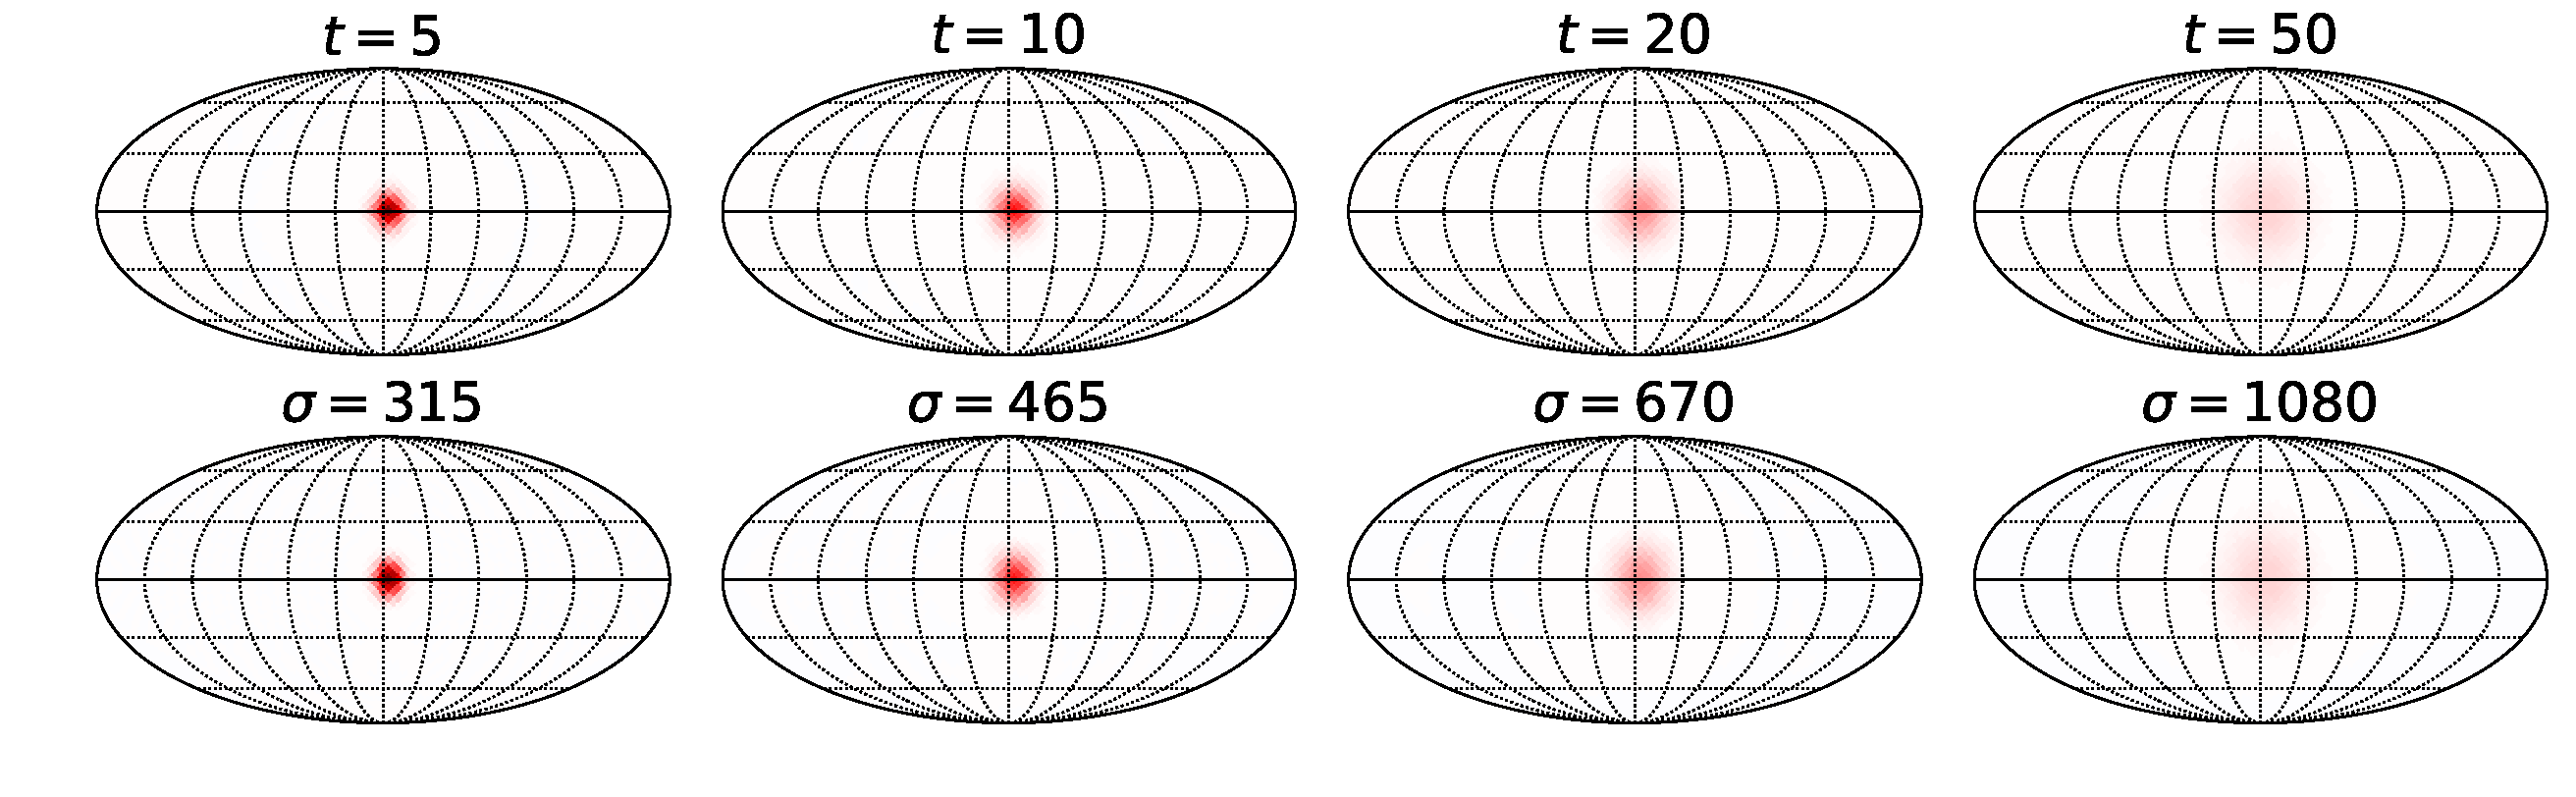
\includegraphics[width=0.95\textwidth]{figures/gaussian_filters_sphere.pdf}
\caption{Convolution comparison (Nside=16).
Top: Diffusion of a unit of heat for different times $t$ using the graph.
Bottom: spherical symmetric Gaussian smoothing for different $\sigma$ (arcmin).
Relative difference between graph convolution and spherical smoothing: $10.4$\%, $5.7$\%, $4.8$\%, $3.8$\% }
\label{fig:gaussian_filters_comparizon}
\end{figure*}

This result is another sign that the constructed graph is able to capture the spherical
structure of the HealPix sampling. Furthermore, in some application, where the
exactitude of the convolution is not a requirement, such as de-noising, it means
that we could use the graph convolution instead. Depending on the convolution kernel
this may reveal much more efficient. In the case of a neural network, the fact
that both convolution are not identical is not very relevant since the network
will adapt the convolution at use.

\subsection{Efficient convolutions}
\assign{Michaël}
With the Fourier basis. Because we don't have an FFT, that costs $O(n^3)$ for the eigendecomposition, plus $O(n^2)$ for the transform (to be done for each forward and backward pass).
\begin{itemize}
	\item We need efficient convolution, hence the Chebysheff trick
	\item Explain the different between a polynomial filter convolution and a traditional patch restricted convolution
	\item Define spherical CNN using graph CNN
\end{itemize}


\subsection{Coarsening}
The HealPix sampling presents the advantage to have a natural coarsening method
based on its construction. Each Nside level divides each pixel into 4 subpixels.
We define the pooling process as the inverse operation grouping the 4 subpixels.
Figure~\ref{fig:pooling} illustrates the process.
\begin{figure}[!ht]
\centering
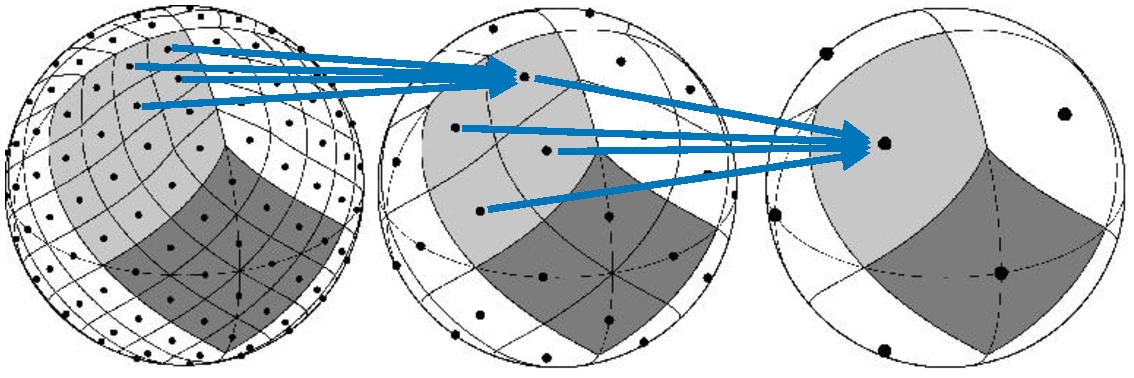
\includegraphics[width=0.45\textwidth]{figures/pooling.pdf}
\caption{Pooling illustration for 2 levels using some part of the mollview projection.
The final patch represents 1/12 of the sphere.}
\label{fig:pooling}
\end{figure}


\section{Experiments}
\label{sec:experiments}

% Structure of the section
% 1) Present the goal
% 2) Explain briefly the dataset
% 3) Present the setting
% 4) Describe the result
In this section, we demonstrate the performance of the spherical neural network on a discrimination problem.
Our implementation is available as a small python package\url{https://our.code.link.com}.
Furthermore, all the data to reproduce our experiments are available online.\footnote{\url{https://doi.org/10.5281/zenodo.????} \todo{correct DOI}}.

In our experiment we classify convergence maps, similar to those created with gravitational lensing technique \citep{chang2017curvedsky}.
We compare the performance of the spherical CNN to a simple benchmark algorithm.
This algorithm is based on classification of histogram of pixels in the maps.
We use an SVM to perform that task.
The benchmark method uses the information about the distribution of pixels, but does not include any spatial information.
The CNN can exploit the spatial information.
The performance is assessed by measuring the classification error on the test set.

Convergence maps represent the dimensionless distribution of over- and underdensities of mass in the universe, projected on the sky plane.
The 3D structures are projected using a geometric kernel, value of which depends on the radial distance.
In gravitational lensing, this kernel is dependent on the radial distances between the observer, the mass plane and the plane of source galaxies \citep[see][for review of gravitational lensing]{bartelman2010gravitationallensing}.
The redshifts of the sources was set to $z=1$.

We make full sky N-body simulations for two parameter set for $\Lambda \rm{CDM} $ cosmological model: model 1 ($\Omega_m=0.31, \sigma_8=0.82$) and model 2 ($\Omega_m=0.26, \sigma_8=0.91$), where $\Omega_m$ is the matter density in the universe and $\sigma_8$ is the normalisation of the matter power spectrum.
Other parameter parameters were set to $h=0.7$ (MORE PARAMS HERE - CHECK WITH RAPHAEL).
These parameters were chosen to have the same spherical harmonic power spectrum for $\ell<1000$.
That means that it is not possible to distinguish between these cosmological models using these maps if the this range of scales is used.
We found that for $\ell>1000$ the differences in power spectrum is $~5\%$.
To remove this information, we additionally smooth the spherical maps with a Gaussian kernel.


\subsection{Data}
\label{sec:data}

The simulations are created using the fast lightcone method described in \citep{sgier2018fastgeneration}.
However, we use only a single simulation box, as opposed to two used in that work, as we use source galaxies at lower redshift of $z=1$, instead of $z=1.5$.
As a simulator we use \pkg{L-PICOLA} \citep{howlett2015lpicola}, a fast and approximate code for N-body simulations.
For each class, we generate 30 simulations.
In the experiment we use data on a parts of the sphere, and we check the performance as a function of the area used.
We also test the performance as a function of noise level of the pixels.

As a pre-processing step, we first remove the mean of each sample and we apply a spherical Gaussian smoothing kernel with a radius of $1$ arcmin.
Out of the 60 simulations, 20 are kept for the test set.
% The training and validation set are created later on.
Figure \ref{fig:map_sample} shows the full sky simulations and a zoom region for model 1 (top) and model 2 (bottom).
Initial conditions for these simulations were the same, so the differences in structures can only be attributed to different cosmological parameters used to evolve the particle distribution.

\begin{figure*}[!ht]
\centering
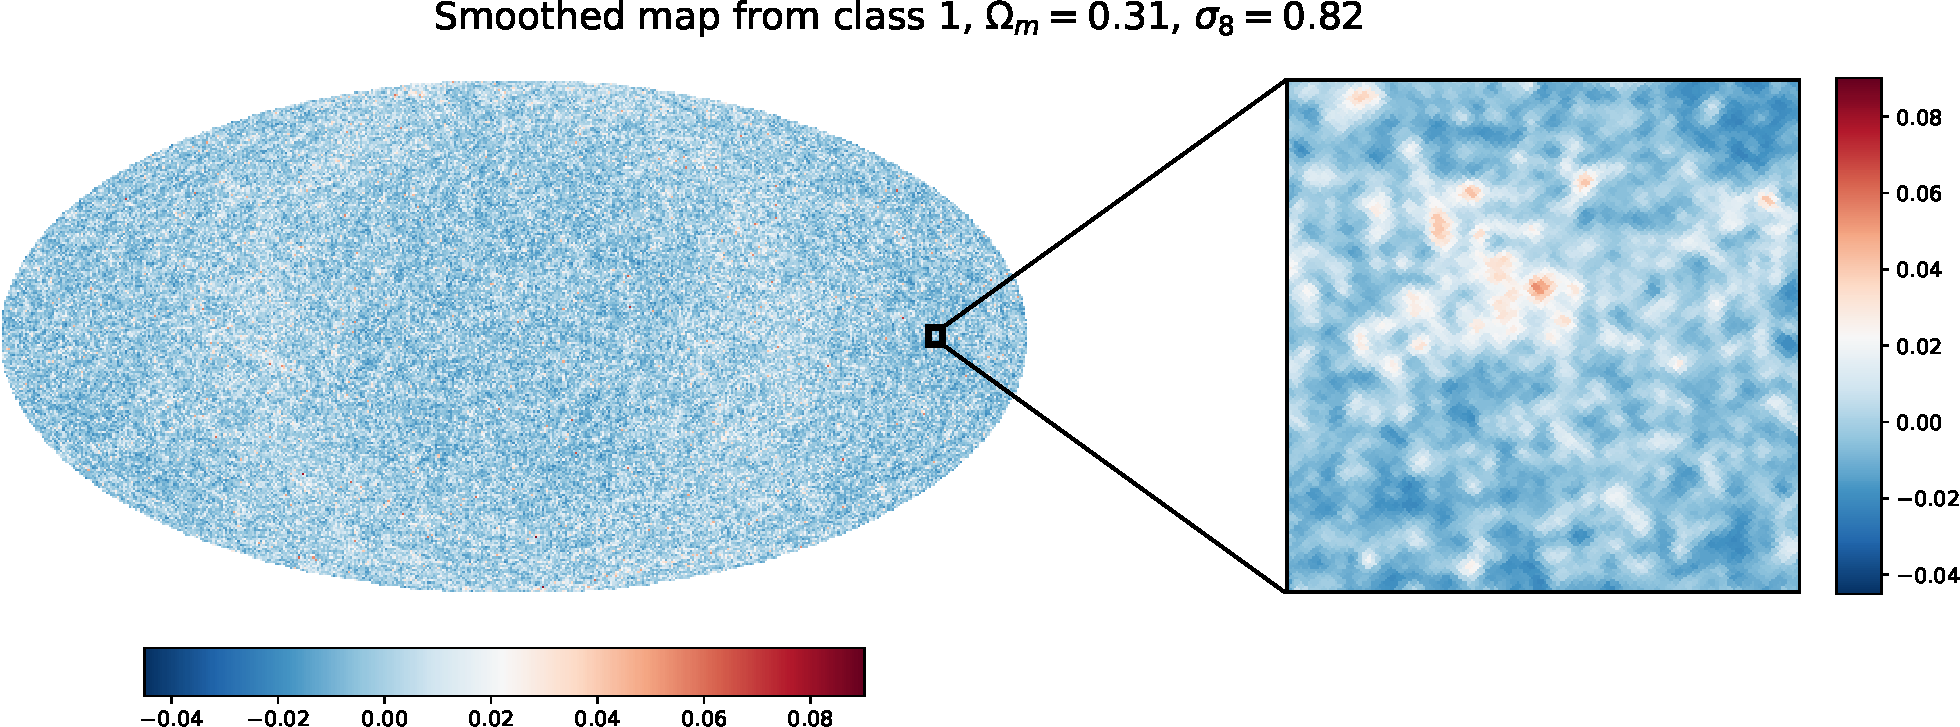
\includegraphics[width=0.95\textwidth]{figures/smooth_map_class_1.pdf}
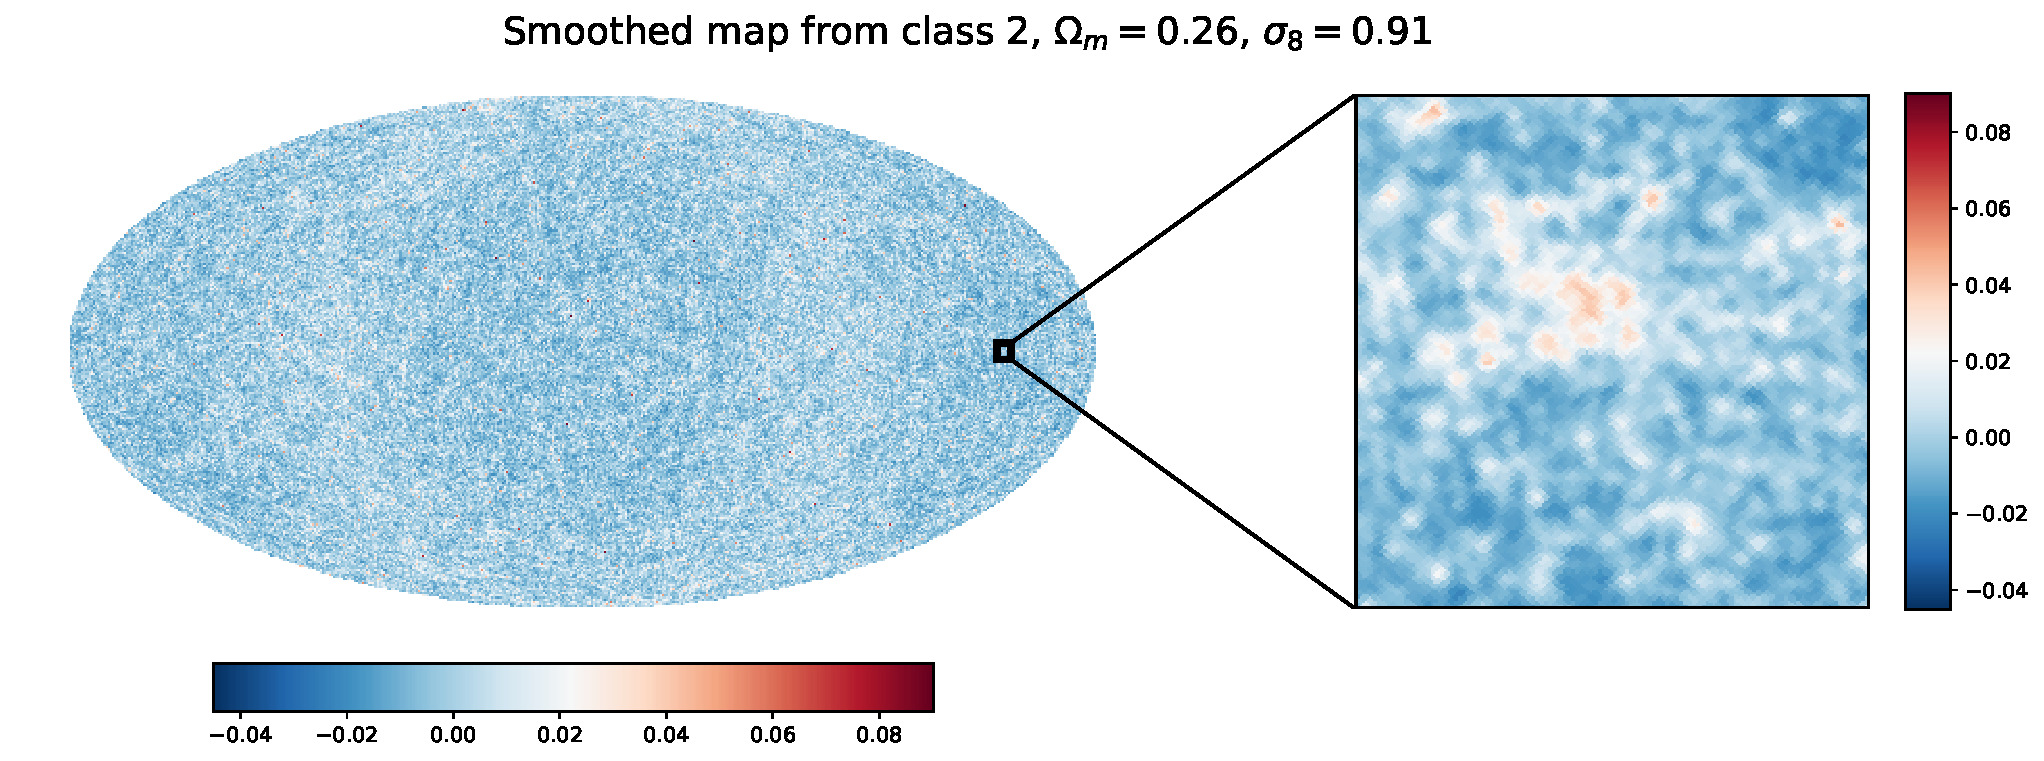
\includegraphics[width=0.95\textwidth]{figures/smooth_map_class_2.pdf}
\caption{Example maps from two classes. Top: model 1 ($\Omega_m=0.31, \sigma_8=0.82$). Bottom: model 2 ($\Omega_m=0.26, \sigma_8=0.91$).
The initial conditions for these simulations were the same, so differences arise only due to different cosmological parameters.}
\label{fig:map_sample}
\end{figure*}

\subsection{Problem formulation}

Leveraging the properties of the HealPix sampling, we can split each simulation
into $12*4^o$ ($o=0,1,2,\dots$) samples that span a smaller part of the sphere.
As shown in Figure~\ref{fig:subpart_sphere}, we used $o=0,1,2$ as the resulting
samples are large enough to suffer from the effects of the spherical geometry. We
decided to only report simulation results for this specific setting as spherical
cosmological data usually does not span the full sphere. Nevertheless, our code
includes an example using the full sphere.

\begin{figure}[!ht]
\centering
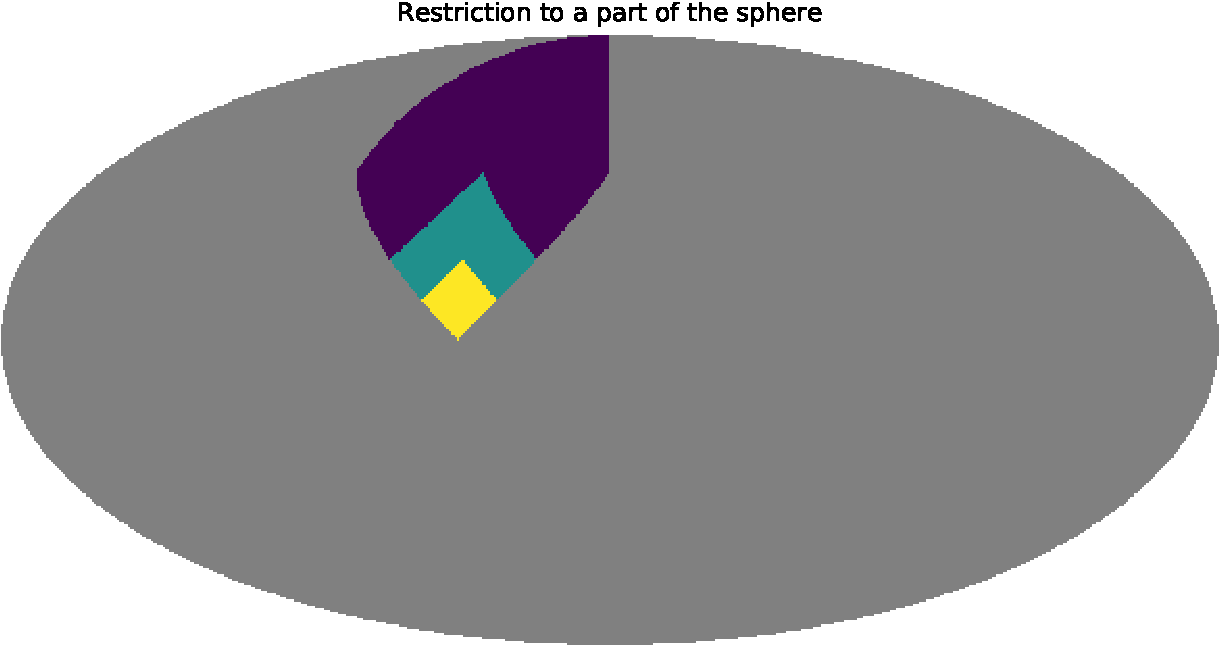
\includegraphics[width=0.45\textwidth]{figures/part_sphere.pdf}
\caption{3 subparts of the sphere with different sizes. Blue: $o=0$. Green: order $o=1$. Yellow: order $o=2$.}
\label{fig:subpart_sphere}
\end{figure}

We would like to build a robust classifier, i.e. an automatic way to
discriminate between the two classes with the presence of noise. For all the
experiments, we work with centered Gaussian noise. \todo{Tomek: could you put a
justification.} All classifiers are trained with noisy samples. To improve the
stability of the spherical CNN, we slowly increase the amount of noise added to
the training data over the iterations. Furthermore in order to avoid
overfitting, the noise is randomly produced during the training process. We trained our
model between $5$ and $40$ epochs depending on the complexity and the size of
the problem. The testing set was simply used to assess the global performance of
the network and to assess if it was overfitting.
Training took between $1$ and $10$ hours using a Nvidia 1080 TI.

We compare the spherical CNN with a handcrafted feature classifier. CITE \cite{...}
\todo{Tomek: we probably need 1 or two other classifiers.} The features are
constructed using a normalized histogram of the values. We then train a linear
SVN classifier. We tried different kernels, but they were not leading to better
results. For a fair comparison, we increase the amount of training data of the
SVN classifier until the testing error plateau to a fix value.

\subsection{Results}
\assign{Nathanaël, Tomek}

We present in Figure~\ref{fig:results} the results for 5 different noise levels and $3$ different data sizes. The spherical neural network is always significantly better than the hand-crafted classifier.

\begin{figure*}[!ht]
\centering
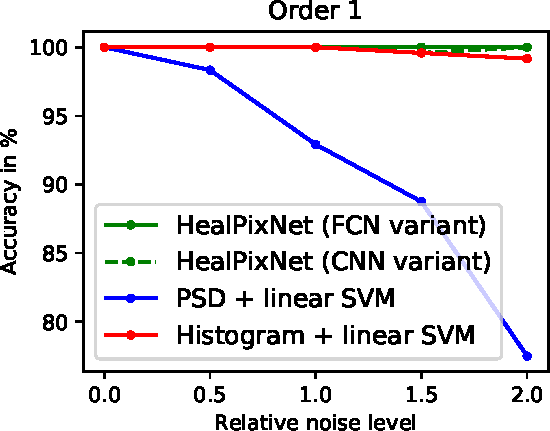
\includegraphics[width=0.32\textwidth]{figures/result_order1.pdf}
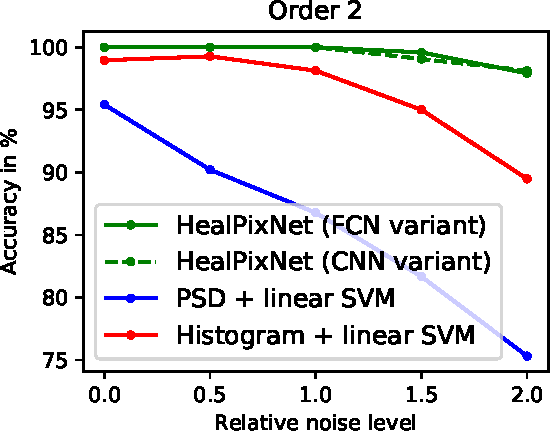
\includegraphics[width=0.32\textwidth]{figures/result_order2.pdf}
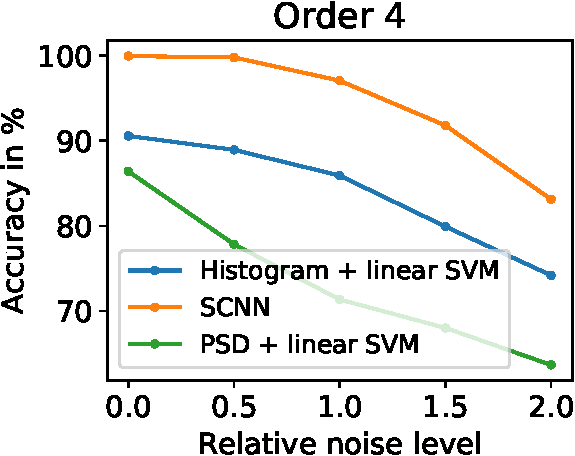
\includegraphics[width=0.32\textwidth]{figures/result_order4.pdf}
\caption{Classification errors for the 3 different problems. \nati{TODO: order is not correct} }
\label{fig:results}
\end{figure*}




\subsection{Interpretation}
\assign{Nathanaël, Tomek, Michaël}

Show the learned filters and feature maps and try to interpret them.
\todo{\\ TK and NP: Figure of filters from the mass map clasification}

Figure: Filters 1D and Gnonomic

\section{Conclusion}
\label{sec:conclusion}
\assign{Nathanaël, Tomek, Michaël}

\section*{Thanks}

%% The Appendices part is started with the command \appendix;
%% appendix sections are then done as normal sections
\appendix

\section{Filter visualization}
\label{app:filter_visualization}

In Figure~\ref{fig:gaussian_filters_visualization}, we present three different
ways to plot the graph convolution kernel $K_t(x)=e^{-\tau t x}$. First, they can
be plotted in the graph spectral domain. In this case, we simply evaluate $K_t$
at the graph eigenvalues $\text{diag}(\bLambda)$. Second, we can convolve a
delta on the sphere and plot a gnomonic view of the results. Third, since we are
working on the sphere, we can only plot the section of the convoluted delta. In
Figure~\ref{fig:index_section}, we display the selected indexes for the section
plotting. Note that, because of the small irregularities in the HealPix
sampling, the second and the third methods are likely to change depending on the
chosen delta.

\begin{figure*}[!ht]
\centering
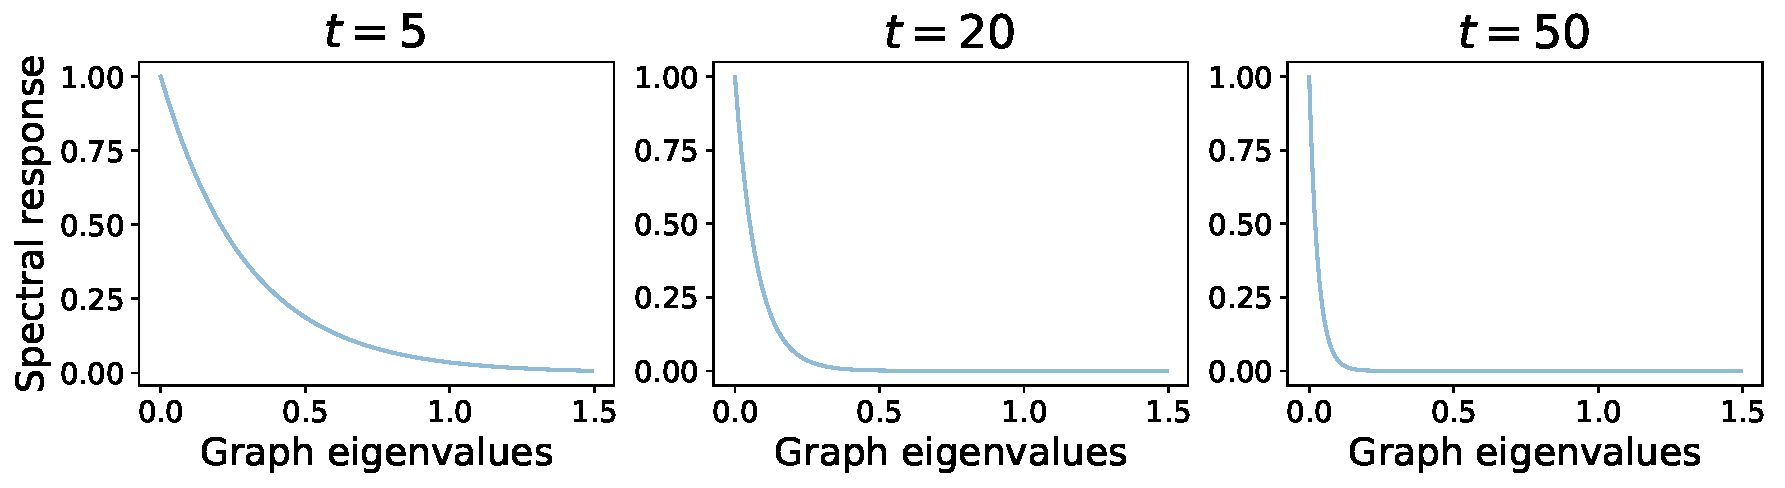
\includegraphics[width=0.95\textwidth]{figures/gaussian_filters_spectral.pdf}
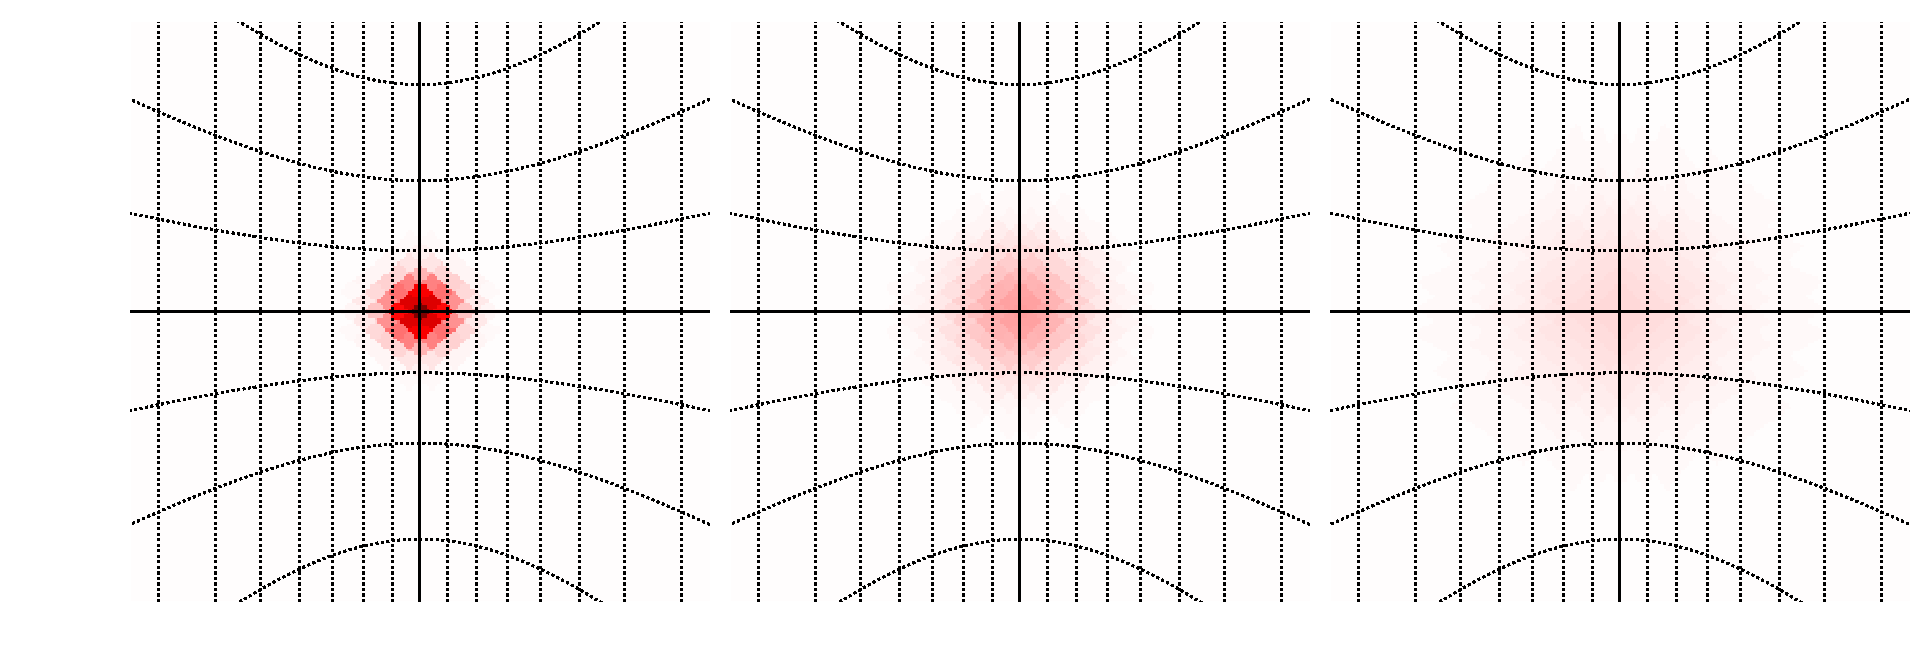
\includegraphics[width=0.95\textwidth]{figures/gaussian_filters_gnomonic.pdf}
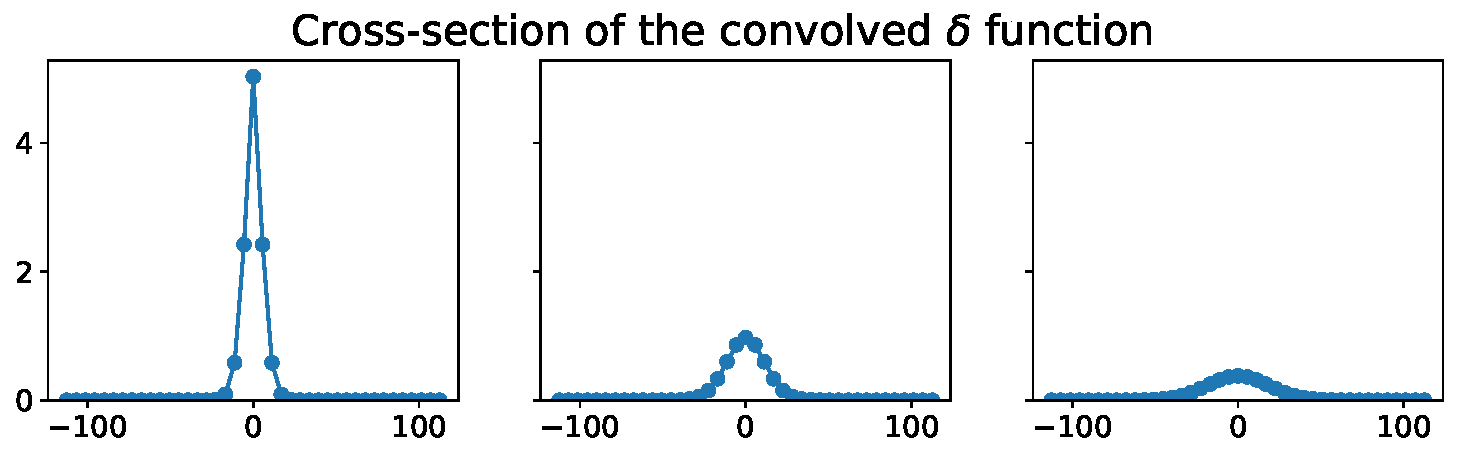
\includegraphics[width=0.95\textwidth]{figures/gaussian_filters_section.pdf}
\caption{3 different visualizations of the convolution kernel $K_t(x)=e^{-\tau t x}$.
Top: graph spectral domain.
Middle: gnomonic projection.
Bottom: section plot.}
\label{fig:gaussian_filters_visualization}
\end{figure*}

\begin{figure}[!ht]
\centering
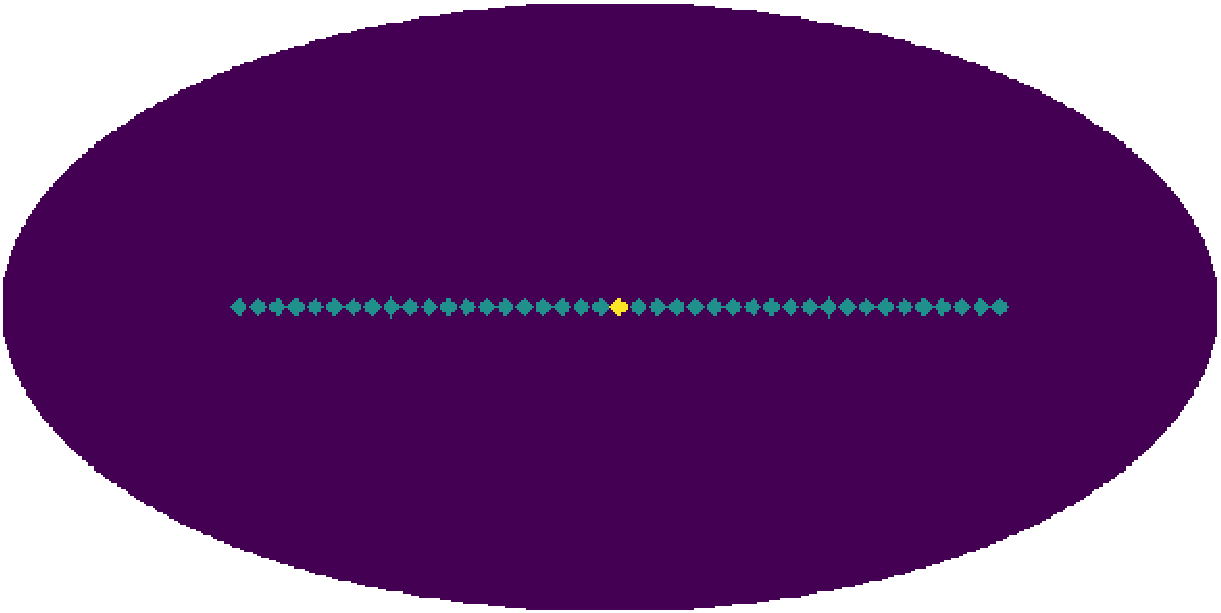
\includegraphics[width=0.45\textwidth]{figures/index_plotting_order20_nside16.pdf}
\caption{Indexes selected for the section ploting of Figure~\ref{fig:gaussian_filters_visualization} middle. The delta was placed on the yellow node.}
\label{fig:index_section}
\end{figure}



%% If you have bibdatabase file and want bibtex to generate the
%% bibitems, please use
%%
\section*{Bibliography}
\bibliographystyle{elsarticle-harv}
\bibliography{biblio}

\end{document}

\endinput
%%
%% End of file `elsarticle-template-harv.tex'.
